\chapter{Erste Standardmodelle der Wahrscheinlichkeitstheorie}

%\subsection{Diskrete Verteilungen}
\section*{Diskrete Verteilungen}

\section{Diskrete Gleichverteilungen}

%TODO restructure! looks like this is just a new section in the chapter Grundbegriffe der Wahrscheinlichkeitstheorie!
% I think that should be a new chapter, but I am not sure what to do with the unnumbered heading "Diskrete Verteilungen", especially headings "Diskrete Gleichverteilungen" and "Urnenmodelle" should have numbers 2.1 and 2.2 (so should be sections)

Erinnerung:
\begin{*erinnerung}[\propref{1_10}]
	Ist $\Omega$ endlich, so heißt Wahrscheinlichkeitsmaß mit Zähldichte
	\begin{align}
		\rho(\omega) = \frac{1}{\omega}\quad, \omega \in \Omega\notag
	\end{align}
	\begriff{(diskrete) Gleichverteilung} auf $\Omega \to U(\Omega)$
\end{*erinnerung}
Es gilt das für jedes $A \in \pows(\Omega)$
\begin{align}
	\probp\brackets{A} = \frac{\abs{A}}{\abs{\Omega}} \notag
\end{align}
Anwendungsbeispiele sind faires Würfeln, fairer Münzwurf, Zahlenlotto, ...

\section{Urnenmodelle}

Ein ``Urnenmodell'' ist eine abstrakte Darstellung von Zufallsexperimenten, bei denen zufällig Stichproben aus einer gegebenen Menge ``gezogen'' werden.
\begin{*definition}[Urne]
	Eine Urne ist ein Behältnis in welchem sich farbige/nummerierte Kugeln befinden, die ansonsten ununterscheidbar sind.
\end{*definition}
Aus der Urne ziehe man blind/zufällig eine oder mehrere Kugeln und notiere Farbe/Zahl.

\begin{center}
%	\documentclass{standalone}

\usepackage{tikz}

\begin{document}
	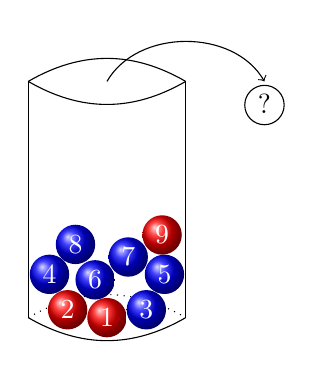
\begin{tikzpicture}
		\draw (0,0) -- (0,-3);
		\draw (2,0) -- (2,-3);
		\draw (0,-3) to [bend right] (2,-3);
		\draw[dotted] (0,-3) to [bend left] (2,-3);
		\draw (0,0) to [bend right] (2,0);
		\draw (0,0) to [bend left] (2,0);
		
		\begin{scriptsize}
		\shade [ball color=red] (1,-3) circle (0.25cm);
		\shade [ball color=red] (0.5,-2.9) circle (0.25cm);
		\shade [ball color=blue] (1.5,-2.9) circle (0.25cm);
		\shade [ball color=blue] (0.27,-2.45) circle (0.25cm);
		\shade [ball color=blue] (1.73,-2.45) circle (0.25cm);
		\shade [ball color=blue] (0.85,-2.52) circle (0.25cm);
		\shade [ball color=blue] (1.27,-2.23) circle (0.25cm);
		\shade [ball color=blue] (0.6,-2.07) circle (0.25cm);
		\shade [ball color=red] (1.7,-1.95) circle (0.25cm);
		\end{scriptsize}
		\node[white] at (1,-3) (1) {1};
		\node[white] at (0.5,-2.9) (2) {2};
		\node[white] at (1.5,-2.9) (3) {3};
		\node[white] at (0.27,-2.45) (4) {4};
		\node[white] at (1.73,-2.45) (5) {5};
		\node[white] at (0.85,-2.52) (6) {6};
		\node[white] at (1.27,-2.23) (7) {7};
		\node[white] at (0.6,-2.07) (8) {8};
		\node[white] at (1.7,-1.95) (9) {9};
		
		\draw[->] (1,0) to [bend left=60] (3,0);
		\draw (3,-0.3) circle (0.25cm);
		\node at (3,-0.29) (a) {?};
	\end{tikzpicture}
\end{document}
%	\caption{Verteilung zu \propref{2_2_6}} 
    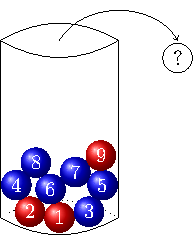
\includegraphics{../../Material/urne_mit_kugeln.pdf}
    \captionof{figure}{Urnenmodell} % needs \usepackage[font=small,labelfont=bf]{caption}
\end{center}

\subsection{Urnenmodell mit Zurücklegen: Multinomial-Verteilung}

Gegeben: Urne mit $N$ Kugeln, verschiedenfarbig mit Farben aus $E$, $\abs{E} \ge 2$ 

Ziehe: $n$ Stichproben/Kugeln, wobei nach jedem Zug die Kugel wieder zurückgelegt wird. Uns interessiert die Farbe in jedem Zug, setze also
\begin{align}
	\Omega = E^n \und \sigF = \pows(\Omega) \notag
\end{align}
Zur Bestimmung einer geeigneten Wahrscheinlichkeitsmaßes, nummerieren wir die Kugeln mit $1,\dots, N$, so dass alle Kugeln der Farbe $a \in E$ eine Nummer aus $F_{a} \subset \set{1,\dots, N}$ tragen. Würden wir die Nummern notieren, so wäre
\begin{align}
	\overline{\Omega} = \set{1,\dots, N}^n \und \overline{\sigF} = \pows(\overline{\Omega})\notag
\end{align}
und wir könnten die Gleichverteilung $\overline{\probp} = \Gleich(\overline{\Omega})$ als Wahrscheinlichkeitsmaß für einem einzelnen Zug verwenden. Für den Übergang zu $\Omega$ konstruieren wir  Zufallsvariablen. Die Farbe im $i$-ten Zug wird beschrieben durch
\begin{align}
	X_i: \overline{\Omega} \to E \mit \overline{\omega} = \left( \overline{\omega}_1, \dots, \overline{\omega}_n \right) \mapsto a \text{ falls } \overline{\omega}_i \in F_a\notag
\end{align}
Der Zufallsvektor
\begin{align}
	X = (X_1, \dots, X_n): \overline{\Omega} \to \Omega\notag
\end{align}
beschreibt dann die Abfolge der Farben. Für jedes $\omega \in \Omega$ gilt dann
\begin{align}
	\set{X = \omega} = F_{\omega_1} \times \cdots \times F_{\omega_n} = \bigtimes_{i=1}^{n} F_{\omega_i}\notag
\end{align}
und damit
\begin{align}
	\probp(\set{\omega}) 
	&= \overline{\probp}(X^{-1}(\set{\omega})) = \probp(X=\omega)\notag\\
	&= \frac{\abs{F_{\omega_1}} \cdots \abs{F_{\omega_n}}}{\abs{\overline{\Omega}}}\notag\\
	&= \prod_{i=1}^{n} \frac{\abs{F_{\omega_i}}}{N} =: \prod_{i=1}^{n} \rho(\omega_i)\notag
\end{align}
Zähldichten, die sich als Produkt von Zähldichten schreiben lassen, werden auch als \begriff{Produktdichten} bezeichnet ($\nearrow$  \S 3 Unabhängigkeit). %TODO ref?!?!?!

Sehr oft interessiert bei einem Urnenexperiment nicht die Reihenfolge der gezogenen Farben, sondern nur die Anzahl der Kugeln in Farbe $a \in E$ nach $n$ Zügen. Dies enspricht
\begin{align*}
	\hat{\Omega} 
	= \set{k = (k_a)_{a \in E} \in \N_{0}^{\abs{E}} \colon \sum_{a \in E} k_a = n}
	\und \hat{\sigF} = \pows\brackets{\hat{\Omega}}\\
	\intertext{Den Übergang $\Omega \to \hat{\Omega}$ beschreiben wir durch die Zufallsvariablen}
	Y_a(\omega): \Omega \to \N_{0} \mit \omega &= (\omega_1,\dots, \omega_n)\mapsto \sum_{a \in E} \indi_{\set{a}}(\omega_i)\\
	\intertext{und}
	Y = \brackets{Y_a}_{a\in E}: \Omega \to \hat{\Omega} &= \set{k = (k_a)_{a\in E}\colon \sum_{a \in E} k_a = n}
\end{align*}

% % % % % % % % % % % % % % % % % % % % 4th lecture % % % % % % % % % % % % % % % % % % % % % % %

Wir erhalten
\begin{align*}
	\probp(Y = k) &= \probp(Y_a = k_a, \enskip a \in E)\\
	&= \sum_{\omega \in \Omega: Y(\omega) = k} \prod_{i=1}^{n} \rho(\omega_i)\\
	&= \sum_{\omega \in \Omega: Y(\omega) = k} \prod_{a \in E} \rho(a) = \binom{n}{(k)_{a\in E}} 
%	\begin{pmatrix}
%	n \\
%	(k)_{a\in E}
%	\end{pmatrix}
	\prod_{a \in E} \rho(a)^{k_a}\\
	\intertext{wobei}
	\binom{n}{(k_1, \dots, k_l)} &= 
	\begin{cases}
	\frac{n!}{k_1 ! \, k_2 ! \cdots k_l !} \sum_{i=1}^{l} k_i = n\\
	0 & \sonst
	\end{cases}
\end{align*}
der \begriff{Multinomialkoeffizient} ist, welcher die Anzahl der Möglichkeiten beschreibt, $n$ Objekte in $l$ Gruppen aufzuteilen, so dass Gruppe $i$ gerade $k_i$ Objekte beinhaltet.

\begin{definition}
	Sei $l > 2, p = (p_1, \dots, p_l)$ eine Zähldichte und $n \in \N$, dann heißt die Verteilung auf \\
	$\set{k = (k_i)_{i=1,\dots,l} \in \N_{0}^{l} : \sum_{i=1}^{l} k_i = n}$ mit Zähldichte
	\begin{align}
		m((k_1,\dots,k_l)) = \binom{n}{k_1, \dots, k_l}\prod_{i=1}^{l} p_i^{k_i}\notag
	\end{align}
	\begriff{Multinomialverteilung mit Parametern $n$ und $p$}. Wir schreiben auch $\Multi(n,p)$.
\end{definition}

\begin{example}
	Eine Urne enthalte nur schwarze ``$1$'' und weiße ``$0$'' Kugeln, d.h. $E=\set{0,1}$, und es sei $\rho(1) = p$ gerade die Proportion der schwarzen Kugeln (= Wahrscheinlichkeit bei einem Zug schwarz zu ziehen), dann ist Wahrscheinlichkeit in $n$ Zügen $k$-mal schwarz zu ziehen:
	\begin{align}
		\binom{n}{k}\prod_{i=0,1} \rho(i)^{k_i} = \binom{n}{k} p^k (1-p)^{n-k}.\notag
	\end{align}
	Ein solches (wiederholtes) Experiment mit nur zwei möglichen Ereignissen und fester Wahrscheinlichkeit $p \in [0,1]$ für eines der Ergebnisse nennen wir auch \begriff{(wiederholtes) Bernoulliexperiment}.
\end{example}

\begin{definition}
	Sei $p \in [0,1]$ und $n \in \N$, dann heißt die Verteilung mit Zähldichte
	\begin{align}
		\rho(k) = \binom{n}{k}p^k (1-p)^{n-k} \mit k \in \set{0,1,\dots,n}.\notag
	\end{align}
	\begriff{Binomialverteilung auf $\set{0, \dots,n}$ mit Parameter $p$} (auch \begriff{Erfolgswahrscheinlichkeit}). Wir schreiben auch $\Bin(n,p)$. Im Fall $n = 1$ nennen wir die Verteilung mit Zähldichte
	\begin{align}
		\rho(0) = 1-p \und \rho(1) = p\notag
	\end{align}
	auch \begriff{Bernoulliverteilung mit Parameter $p$} und schreiben $\Ber(p)$.
\end{definition}
\underline{Urnenmodell ohne Zurücklegen}: \begriff{Hypergeometrische Verteilung}\\
Gegeben: Urne mit $N$ Kugeln verschiedener Farben aus $E$,
\begin{align}
	\abs{E} \ge 2.\notag
\end{align}
Es werden $n \le N$ Stichproben entnommen, wobei die gezogenen Kugeln werde \emph{nicht} in die Urne zurückgelegt.

\subsection{Urnenmodell ohne Zurücklegen: Hypergeometrische Verteilung}
Gegeben: Urne mit $N$ Kugeln verschiedener Farben aus $E$, $\abs{E} \ge 2$. Es werden $n \le N$ Stichproben entnommen, wobei die gezogenen Kugeln werde \emph{nicht} in die Urne zurückgelegt.
\begin{example}
	Eine Urne enthalte $S$ schwarze ``$1$'' und $W$ weiße Kugeln ``$0$'' Kugeln, $(E = \set{0,1}, S + W =N)$. Dann ist die Wahrscheinlichkeit in $n$ Zügen ohne Zurücklegen gerade $s$ schwarze und $w$ weiße Kugeln zu ziehen
	\begin{align}
		\rho(w) = \frac{\binom{W}{w}\binom{S}{s}}{\binom{N}{n}}, \quad 0 \le s \le S, 0 \le w \le W, s+w = n, S+W = N.\notag
	\end{align}
\end{example}

\begin{proof}
	Hausaufgabe! %TODO add number later
\end{proof}

\begin{definition}
	Seinen $N \in \N, W \le N, n \le N$, dann heißt die Verteilung auf $\set{0,\dots,n}$ mit Zähldichte
	\begin{align}
		\rho(w) = \frac{\binom{wW}{w}\binom{N-W}{n-w}}{\binom{N}{n}}, \quad w = \max\set{0,n=N+W}, \dots, \min\set{W,n},\notag
	\end{align}
	die \begriff{Hypergeometrische Verteilung} mit Parametern $N,W,n$. Wir schreiben $\Hyper(N,W,n)$.
\end{definition}

\section{\person{Poisson}-Approximation und \person{Poisson}-Verteilung}

$\Bin(n,p)$ ist zwar explizit und elementar definiert, jedoch für große $n$ mühsam auszuwerten. Für seltene Ereignisse ($n$ groß, $p$ klein) verwende daher:
\begin{proposition}[Poisson-Approximation]
	Sei $\lambda > 0$ und $(p_n)_{n\in\N}$ eine Folge in $[0,1]$ mit
	\begin{align}
		np_n \to \lambda,\quad n \to \infty.\notag
	\end{align}
	Dann gilt $\forall k \in \N_0$ für die Zähldichte der $\Bin(n,p_n)$-Verteilung
	\begin{align}
		\lim_{n \to \infty} \binom{n}{k}p_n^k(1-p)^{n-k} = e^{-\lambda} \frac{\lambda^k}{k!}.\notag
	\end{align}
\end{proposition}
\begin{proof}
	Sei $k \in \N_{0}$ fix, dann
	\begin{align} %TODO fix this alignment mess and the tags!
		\binom{n}{k} = \frac{n!}{k!(n-k)!} &= \frac{n^k}{k!}\frac{n(n-1)\cdots(n-k+1)}{n^k}\notag\\
		&= \frac{n^k}{k!}\cdot 1 \cdot (1-\frac{1}{n}\cdots \frac{k-1}{n})\notag\\
		\overset{n \to \infty}&{\sim} \frac{n^k}{k!},\notag
	\end{align}
	wobei $a(l) \overset{n \to \infty}{\sim} b(l) \Leftrightarrow \frac{a(l)}{b(l)} \xrightarrow{n\to \infty} 1$. Damit
	\begin{align}
		\binom{n}{k}p^k (1-p)^{n-k} \overset{n \to \infty}&{\sim} \frac{n^k}{k!}p_n^k(1-p_n)^{n-k}\notag\\
		\overset{n \to \infty}&{\sim} \frac{\lambda^k}{k!}(1-p_n)^n\notag\\
		&= \frac{\lambda^n}{k!}\brackets{1 - \frac{np_n}{n}}^n\notag\\
		&\xrightarrow{n \to \infty} \frac{\lambda^n}{k!}e^{-\lambda}.\notag
	\end{align}
\end{proof}
Der erhaltene Grenzwert liefert die Zähldichte auf $\N_{0}$, denn 
\begin{align}
	\sum_{k=0}^{\infty}\frac{\lambda^k}{k!}e^{-\lambda} = e^{-\lambda}\sum_{k=0}^{\infty}\frac{\lambda^{k}}{k!} = e^{-\lambda}e^{\lambda} = 1\notag
\end{align}

\begin{definition}
	Sei $\lambda >0$. Dann heißt das auf $(\N_{0}, \probp(\N_{0}))$ definierte Wahrscheinlichkeitsmaß mit
	\begin{align}
		\probp(\set{k}) = \frac{\lambda^k}{k!}e^{-\lambda} \quad k \in \N_{0},\notag
	\end{align}
	\begriff{Poissonverteilung mit Parameter $\lambda$}. Schreibe $\Pois(\lambda)$.
\end{definition}
Die Poissonverteilung ist ein natürliches Modell für die Anzahl von zufälligen, seltenen Ereignissen (z.B. Tore im Fußballspiel, Schadensfälle einer Versicherung, ...).